\documentclass[a4,center,fleqn]{NAR}

% without these packages \url won't work:
\usepackage{url}  
\usepackage{hyperref} 

\usepackage{pdfpages}
% to cross reference SI figures !! DOES NOT WORK
%\usepackage{xr} 
%\externaldocument{manuscriptSI}

%% macros
  \newcommand{\dd}{\mathrm{d}}

  \newcommand{\ti}{r_\textsl{ti}}
  \newcommand{\tv}{r_\textsl{tv}}
  \newcommand{\pa}{\pi_\textrm{A,T}}
  \newcommand{\pc}{\pi_\textrm{C,G}}
  \newcommand{\pbbis}{\pi_\textrm{b}}
  \newcommand{\pbp}{\pi_\textrm{b'}}

  \newcommand{\wb}{w_\textrm{b}}
  \newcommand{\wbp}{w_\textrm{b'}}

  \newcommand{\fat}{t_{A\rightarrow T}}
  \newcommand{\fac}{t_{A\rightarrow C}}
  \newcommand{\fag}{t_{A\rightarrow G}}
  \newcommand{\fta}{t_{T\rightarrow A}}
  \newcommand{\ftc}{t_{T\rightarrow C}}
  \newcommand{\ftg}{t_{T\rightarrow G}}
  \newcommand{\fca}{t_{C\rightarrow A}}
  \newcommand{\fct}{t_{C\rightarrow T}}
  \newcommand{\fcg}{t_{C\rightarrow G}}
  \newcommand{\fga}{t_{G\rightarrow A}}
  \newcommand{\fgt}{t_{G\rightarrow T}}
  \newcommand{\fgc}{t_{G\rightarrow C}}
  \newcommand{\fbbp}{f_{b,b'}}
  \newcommand{\fbpb}{f_{b',b}}

  \newcommand{\proba}{\mathcal{P}}

  \newcommand{\neff}{\mathcal{N}_\mathrm{eff}}


  \newcommand{\Ham}{\mathcal{H}}


  \newcommand{\sensillum}{\emph{sensillum}}
  \newcommand{\sensilla}{\emph{sensilla}}

  \newcommand{\droso}{\emph{Drosophila melanogaster}}
  \newcommand{\drosim}{\emph{D. melanogaster}}
  \newcommand{\celeg}{\emph{Caenorhabditis elegans}}
  \newcommand{\csim}{\emph{C. elegans}}

  \newcommand{\mfl}{\emph{mixed feedback loop}}
  \newcommand{\etal}{\emph{et al}}
  \newcommand{\ecoli}{\emph{E. coli}}
  

% Enter dates of publication
\copyrightyear{}
\pubdate{}
\pubyear{}
\jvolume{}
\jissue{}

%\articlesubtype{This is the article type (optional)}

\begin{document}

\title{Imogene: identification of motifs and cis-regulatory modules
underlying gene co-regulation}

\author{%
Herv\'e Rouault\,$^{1,2,+,*}$,
Marc Santolini\,$^{3,+}$,
Fran\c{c}ois Schweisguth\,$^{1,2}$ and
Vincent Hakim\,$^3$%
\footnote{To whom correspondence should be addressed.
 Email: vincent.hakim@ens.fr}}

\address{%
$^{1}$ Institut Pasteur, Developmental Biology Department,75015 Paris,
    France,
    $^{2}$CNRS, URA2578, F-75015 Paris, France,
$^{3}$Laboratoire de Physique Statistique, CNRS, \'Ecole Normale Sup\'erieure,
    Universit\'e P. et M. Curie, Universit\'e Paris-Diderot,\\
 $^+$ Have contributed equally\\
$^*$ present address: Janelia Farm Research Campus, Howard Hughes Medical
Institute, Ashburn, VA 20147, USA
}
% Affiliation must include:
% Department name, institution name, full road and district address,
% state, Zip or postal code, coun%\history{%
%Received January 1, 2009;
%Revised February 1, 2009;
%Accepted March 1, 2009}

\maketitle

\begin{abstract}
Cis-regulatory modules (CRMs) and motifs play a central role in tissue and
condition-specific gene expression.
Their identification could be facilitated by the development of suitable
bio-informatic tools.
Here we present {\em Imogene} an ensemble of statistical tools that we have
developed and implemented in a publicly available software.
Starting from a small training set of mammalian or fly CRMs that drive similar
gene expression profiles, {\em Imogene} determines {\em de novo} cis-regulatory
motifs that underlie this co-expression.
It can then predict on a genome-wide scale other CRMs with a regulatory
potential similar to the training set.
{\em Imogene} bypasses the need of large data sets for statistical analyses by
making central use of the information provided by the sequenced genomes of
multiple species, based on the developed statistical tools and explicit models
for transcription factor binding site evolution.
We test {\em Imogene} on characterized tissue-specific mouse developmental
CRMs.
Its ability to identify CRMs with the same specificity based on its {\em de
novo} created motifs equals that of the previously evaluated best motif-blind
methods.
We further show, both in flies and in mammals, that {\em Imogene de novo}
generated motifs are sufficient to discriminate CRMs related to different
developmental programs.
Notably, {\em Imogene} performs as well in this discrimination task purely
based on sequence data, than a previously reported learning algorithm based on
ChIP data for multiple transcription factors.
We thus expect {\em Imogene} to be a useful tool to decipher transcriptional
gene regulation in higher eukaryotes.
\end{abstract}


\section{Introduction}

The identification and functional characterization of the non-coding sequences
that direct the spatio-temporal specificity of gene expression in eukaryotes is
of fundamental importance in developmental biology~\cite{Davidson:2006kx} and
can find crucial applications in medicine~\cite{Dorer:2009wd}.
These regulatory sequences are generally located distally from gene promoters
and termed enhancers or more generically cis-regulatory modules (CRMs) since
they can either enhance or repress gene expression~\cite{pmid22705667}.
They usually are of the order of 500 nucleotides (nts) long and can be located
as far as several mega base-pairs away from the transcription start sites
(TSSs) of the genes that they regulate.
CRMs are composed of transcription factor binding sites (TFBSs) which bring
spatio-temporal specificity to the expression of their target
promoters~\cite{lellimann13arg}. 
Detailed studies in both flies and vertebrates~\cite{levine10cb} have shown
that CRMs contain multiple binding sites for transcription factors (TFs) that
can be either identical (homotypic clustering) or different (heterotypic
clustering).
Homotypic clustering can provide cooperative TF binding and sharp on-off gene
expression whereas heterotypic clustering allows for combinatorial gene
regulation.
The extent to which the order and relative positioning of the different TFBSs
in CRMs matter, remains however debated~\cite{Arnosti:2005uq,Swanson:2010ai}.

With the advent of ChIP-seq techniques, genome-wide studies are providing large
amount of data on the binding loci of tissue-specific transcription
factors~\cite{Johnson:2007fk}, as well as on other factors that regulate
transcription e.~g. by modifying chromatin structure (p300, CTCF, histone
marks, etc)~\cite{Barski:2007uq,Mikkelsen:2007kx}.
This protein binding data has helped 
the identification of numerous CRMs specific to well-defined
developmental processes and it has brought important information  on CRM
structure.
However, genome wide studies suffer from  limitations.
A full characterization of regulatory mechanisms would require ChIP-seq
analysis to be performed for every potential regulatory factor, on every
tissue, at multiple developmental stages.
The results would also have to be obtained for the often heterogeneous cells
that constitute the tissue of interest instead of being averaged over them as
it usually needs to be the case. 
Finally, and very importantly, binding cannot be equated to functional
regulation.

% **************************************************************
% Keep this command to avoid text of first page running into the
% first page footnotes
\enlargethispage{-65.1pt}
% **************************************************************

Therefore, {\em in silico} identification of CRMs  forms a useful complement to
genome-wide binding studies. 
Classic case-by-case studies or large scale binding data~\cite{Visel:2009fr},
as  previously described, often provide a moderate number (about ten to a few
tens) of CRMs, active  in the co-regulation of a subset of genes, in specific
biological systems or in the formation of different  organs at various stages
of development. 
Identifying the important binding sites on these known sequences would help to
bypass some of the limitations of large scale studies by providing information
on the factor involved, both known and new, as well as on the existence of
a regulatory grammar~\cite{arnosti}.
It should also help one to determine other CRMs providing specific expression
patterns, a difficult task at present given the absence of close
association~\cite{pmid19097946} between CRMs and their target genes in higher
eukaryotes.
These labor-intensive experimental tasks could be eased by computational work.
To this end,  we have previously developed~\cite{Rouault:2010fk} statistical
tools to determine cis-regulatory elements \textit{de novo}, in a set of input
DNA sequences encoding a common transcriptional regulation.
They allow the determination of regulatory elements from input DNA sequences
without any  prior information on the transcription factors acting in cis or on
their binding sites. 
They make  central use of  the phylogenetic information
contained in the aligned DNA sequences of related species.
The method was applied to the {\em D. melanogaster} gene expression program in
sensory organ precursor cell (SOPs), a specific type of neural progenitor
cells~\cite{Rouault:2010fk}.
Predicted motifs  included already characterized TFBS as well as new motifs and
were successfully tested by mutational analysis.
These motifs were used to rank intergenic DNA fragments genome wide for their
regulatory potential in SOPs.
Of the top 29 predicted CRMs, 38\% were found by transgenic assays to direct
transcription in SOP. A larger fraction (65\%) drove more generally
transcription in neural precursors.
 
This successful application to a {\em Drosophila} transcriptional program led
us to try and extend the method developed in ref.~\cite{Rouault:2010fk}
to the case of mammalian CRMs.
The task of determining cis-regulatory elements is even more difficult for
mammalian genomes  than for  {\em Drosophila} ones since they are an order of
magnitude richer in intergenic
sequences~\cite{Flicek2012fk,clark2007evolution}.
To tackle this challenge, we have developed {\em Imogene}, a computer algorithm
and software that we present here and characterize.
{\em Imogene} predicts:
\begin{enumerate}
\item  cis-regulatory sequences (of about 10 nt long) within a moderate set
  size  of 10-30 CRMs, responsible for specific gene co-regulation, as well as
  a set of Probability Weight Matrices (PWM) or
  motifs~\cite{pmid15131651,stormo1998specificity} characterizing the
  DNA-binding specificity of the associated putative factors.
\item novel CRMs at the genomic scale with the same expression pattern as the
  starting set of CRMs, based on the set of build PWMs.
\end{enumerate}

Numerous algorithms have already been developed to try and map cis- underlying
transcriptional regulation (see
e.g.~\cite{pmid22705667,pmid21152003,pmid17053094,pmid15131651,pmid22305161}
for recent reviews).
{\em Imogene} differs from previous methods in several respects.
{\em Imogene} aim is most similar to the goal of the algorithms analyzed
in~\cite{kantorovitz2009motif}. 
These algorithms have been specially designed to decode cis-regulatory
regulation in a small set of CRMs,  contrary to  other algorithms which are
aimed at the analysis of large datasets such as whole ChIP-seq peak
regions~\cite{pmid21486936}.
Both work {\em de novo} instead of using already characterized binding
motifs~\cite{berman2002exploiting, halfon2002computation,
  rebeiz2002score,schroeder2004transcriptional, Moses:2004vn,
  siddharthan2005phylogibbs, hallikas2006genome, pierstorff2006identifying,
Herrmann2012uq}.
Faced to the weak statistical discriminative power offered by the starting set
of characterized CRMs, the best algorithms of ref.~\cite{kantorovitz2009motif}
try and distinguish regulatory sequences by their entire content in short
nucleotide sequences as also proposed in other
works~\cite{nazina2003statistical, abnizova2005some, chan2005using,
leung2009identifying, Brody:2012pd}.
On the contrary, {\em Imogene} insists on building cis-regulatory motifs since
those are important for experimental work.
It instead relies on conservation and the comparison of multiple sequenced
genomes.

In the following, the general methodology of {\em Imogene} is first presented.
Then, {\em Imogene} performance on mammalian CRMs is assessed.
Imogene is trained on CRMs pertaining to  neural tube and limb developmental
programs during embryogenesis.
It is shown to successfully classify other CRMs in the same class based on its
{\em de novo} created list of best motifs which contained both new and already
known motifs. 
We then consider the distinct but related task of discriminating CRMs with
different specificities, rather than discriminating a set of specific CRMs from
background intergenic sequences.
{\em Imogene} is shown to accurately discriminate mammalian neural tube from
limb CRMs on the basis of very few learned motifs.
To further assess the performance of {\em Imogene}, it is applied to the
discrimination of five sets of  mesodermal fly CRMs, a task previously
considered in ref.~\cite{pmid19890324}.
The CRM classification solely based on {\em Imogene} {\em de novo} generated
motifs is found to be of similar quality as the results obtained in
ref.~\cite{pmid19890324} based on ChIP binding data for multiple transcription
factors at several developmental time points.
Finally, the developed publicly available {\em Imogene}  interface is
presented.




\section{MATERIALS AND METHODS}

\subsection*{Genome alignments}
The alignments were downloaded from
\url{ftp://ftp.ensembl.org/pub/release-63/emf/ensembl-compara/epo_12_eutherian}
for mammals and from \url{http://www.biostat.wisc.edu/~cdewey/fly_CAF1/data}
for Drosophilae.
For the latter case, we have used the alignments engineered by A. Caspi with
the help of the Mercator and MAVID programs.
In both cases, the alignments were processed through a customized script to
produce alignments in fasta format, mask for coding sequences (CDS) and simple
repeats (see below).
These scripts are available in the {\em Imogene} distribution.

\subsection*{Annotations}
The CDS coordinates were downloaded from
\url{ftp://ftp.ensembl.org/pub/release-64/gtf/mus_musculus} for mammals (mm9
coordinates) and from
\url{ftp://ftp.flybase.net/releases/FB2011_06/dmel_r5.38/gff} for Drosophilae
(release $5$ coordinates).
In the case of mammals, the TSS coordinates were obtained separately from
\url{http://hgdownload.cse.ucsc.edu/goldenPath/mm9/database}.
Mammalian alignments  were already masked for repeat sequences.
Drosophilae alignments were masked using the coordinates indicated in the
\textit{gff} file.

\subsection*{Phylogenetic trees} 

The phylogenetic trees used within {\em Imogene} are displayed in
Figure~\ref{fig:tree}.
For drosophilae, the distances are taken from Heger and
Pontig~\cite{pmid18039870}.
For mammals, they are obtained from the Ensembl  ~\cite{Flicek2012fk}
website
(\url{www.ensembl.org}).


\subsection*{Background sequences}

\textit{Imogene} computes  the statistical over-representation of the predicted
motifs by comparing them to 20 Mb of background intergenic DNA ($10^4$ regions
of $2$ Kb).
The script that generates the  random coordinates is included in the
distribution of {\em Imogene} as well as the actual coordinates of the produced
intergenic regions.

\subsection*{Training sets}
The two used mammalian training sets (limb, neural tube) were obtained from
\url{http://enhancer.lbl.gov}, based on the work
of~\cite{Visel:2009fr,pmid22138689}.
They were manually curated to produce a high-quality data set, with
respectively $41$ CRMs for the limb, and $33$ for the neural tube.
We further pruned out uninformative CRMs for which no motifs could be generated, 
either because of repeat masking or because of lack of conservation.
More precisely, the reference species sequence was scanned using a window size
corresponding to the motif size.
If a sequence did not contain any masked nucleotide, we looked in the other
species for any unmasked sequence in the surrounding neighborhood of $\pm20$nt,
our flexibility criterion when defining a conserved instance.
If putative orthologous sequences were found in enough species to satisfy our
conservation requirements (see below), the site was declared as a putative
conserved site for a regulatory motif. This filtering step resulted in final
sets of  $39$ limb CRMs (minimal length $789$ bp, maximal length $9052$ bp,
average length $3045$ bp) and $29$  neural tube CRMS (minimal length $585$ bp,
maximal length $3045$ bp, average length $2419$ bp).

The Drosophilae training sets were obtained from~\cite{pmid19890324}.
Coordinate files are given as Supplementary Material.



\subsection*{Main program}

The main program is written in C++ and adapted from the program used in
a previous study~\cite{Rouault:2010fk}.
It is distributed under the GNU GPL license and available as a git repository
at \url{http://github.com/hrouault/Imogene}.
The user manual is available at \url{http://hrouault.github.io/Imogene/}.
The program can be accessed through a web
interface at \url{http://mobyle.pasteur.fr/cgi-bin/portal.py#forms::imogene}.

\subsection*{Binding site scores}

A given motif is represented by a PWM with frequency $w_{i,b}$ for the base $b$
at position $i$.
The index $i$ runs from $1$ to $l_m$ the size of the motif which is a parameter
in the program which takes the same value for all considered motifs.
The binding score of a sequence $s_i$ for such a motif, is defined through the
corresponding PWM as:
\begin{equation}
    S=\sum_{i}\log_2\left(\frac{ w_{i,s_i}}{\pi_b}\right)
    \label{score_bs}
\end{equation}
where $\pi_b$ is the mean frequency of  the base $b$ within intergenic regions
($\pa=0.30$ and $\pc=0.20$) as measured on the ``background sequences'' (see
methods {\em Background sequences } subsection for their detailed description).
A sequence is considered as a binding site in the reference species ({\em D.
melanogaster} or  {\em Mus musculus}) when its score $S$ is larger than the
score threshold ($S_s$ or $S_g$) defined by the user of \textit{Imogene}.

\subsection*{Conservation requirements for binding sites} 
{\em Imogene} iteratively builds PWM from binding sites that have conserved
instances in different species.
The conservation requirement is that orthologous instances are found in at
least 3 distant species, including the reference species.
For mammals, the 5 following groups of related species are composed of: {\em
Mus musculus} and {\em Rattus norvegicus}; {\em Callithrix jacchus}, {\em
Macaca mulatta}, {\em Pongo abelii}, {\em Gorilla gorilla}, {\em Homo sapiens}
and {\em Pan troglodytes};  {\em Bos taurus}; {\em Sus scrofa}; {\em Canis
familiaris}; {\em Equus caballus}.
Similarly for flies, there are $5$ groups composed of:
{\em Drosophilae} {\em melanogaster}, {\em sechellia}, 
{\em simulans}, {\em yakuba} and {\em erecta};
{\em Drosophila} {\em ananassae};
{\em Drosophilae} {\em pseudoobscura} and {\em persimilis};
 {\em Drosophila} {\em willistoni};
 {\em Drosophilae} {\em grimshawi}, {\em mojavensis} and {\em virilis}.

A site instance must be found in at least 3 of these 5 groups (with an allowed
shift of up to 20 nt with the reference species) considered conserved by {\em
Imogene}.


\subsection*{Evolutionary models}

{\em Imogene} can use two different evolutionary models, which vary in
complexity and computational time, to compare orthologous binding sites.
In both models, the bases within a site evolve independently from each other. 
\\

\paragraph{Felsenstein model. }

The simplest models of TFBS nucleotides evolution are copied on models of
neutral evolution for genomic nucleotides.
This procedure has been proposed by Sinha \textsl{et al}~\cite{Sinha:2003vn,
siddharthan2005phylogibbs}  with the Felsenstein model of neutral
evolution~\cite{Felsenstein:1981ve}.
In this TFBS evolution model, the transition probability from nucleotide $b$ to
$b'$ at position $i$ in two sites at evolutionary distance $d$ is defined as:
\begin{equation}
    p_{b\rightarrow b'}^i=q\ \delta_{b,b'}+(1-q)\ w_{i,b'}
    \label{felsenstein-integr-TF}
\end{equation}
where $\delta_{b,b'}$ is the Kronecker symbol, $w_{i,b'}$ is the mean frequency
of base $b'$ at position $i$ of the site (as given by the PWM model), and $q$ is
the probability of conservation for an evolutionary distance  $d$ under neutral
selection (see below).

When two species are close to one another, $q\sim1$ and the probability that
the observed bases are identical is high.
On the contrary, when the two considered species are distant ($q\sim0$), the
observed bases are uncorrelated and reflect the PWM probabilities $w_{i,b}$.

The probability of conservation $q$ can then be computed within this model by
setting the PWM probabilities $w_{i,b}$ to the mean genomic frequencies
$\pi_b$:
\begin{equation}
        q=\exp\left(-\frac{d}{1/2+4\pa\pc}\right) \label{q-felsen-TF}
\end{equation}
with $\pa$ (resp. $\pc$) the common genomic frequency of A and T (resp. C and
G).

\paragraph{Halpern-Bruno model. }
The Halpern-Bruno model (HB) \cite{Halpern:1998qf} differs in two ways from the
simplest {\em Felsenstein} model.
It uses  the more complex Hasegawa, Kishino and Yano model
(HKY)~\cite{Hasegawa:1985dp} for the neutral evolution of nucleotides and adds
a fixation probability based on fitness differences for the evolution of
nucleotides within the TFBS.

The HKY model  improves on the Felsenstein model by taking into account the
observed dependence of the mutation rate on the chemical nature of the bases. 
Substitutions between bases of the same chemical nature (purine or pyrimidine),
also called transitions, are generally more frequent than the other type of
mutations, called transversions.
This is encapsulated in the HKY model by the parameter $\kappa$ which is the
ratio of the transition rate over the transversion rate.
It is measured to be $\kappa=2$ in flies and $\kappa=3.7$ in
mammals~\cite{kappa12paper}.  

Within a TFBS, the HB model extends the HKY model to take into account an
additional purifying selection on the nucleotide
identities~\cite{Halpern:1998qf}. 
It is formulated by the following transition probabilities:
\begin{equation}
   p_{b\rightarrow b'}=\exp(t\mathbf{H})_{b,b'}
   \label{HB-integr}
\end{equation}
where $\mathbf{H}$ is the rate matrix defined by:
\begin{equation}
	H_{b,b'} =
	\begin{cases}
		\pi_{b}\ h_{b'\to b} & \text{if } b\neq b'\\
		- \sum_{b'\neq b} H_{b,b'} & \text{if } b = b'
	\end{cases}
   \label{HB-transi}
\end{equation}
The evolutionary time $t$ is expressed in term of the evolutionary distance by:
\begin{equation}
t=\frac{d}{1/2+4\kappa\, \pa\pc}
    \label{rateHKY}
\end{equation}

Finally, the transition rates are defined by:
\begin{equation}
   h_{b\rightarrow b'}=\frac{\wbp}{\pbp}\ \frac{\log\left(\frac{\pbbis \wbp}{\pbp \wb} \right)}{\wbp / \pbp - \wb / \pbbis} \alpha_{b\rightarrow b'}
   \label{fixation-prob-HB model}
\end{equation}
with $\alpha_{b\rightarrow b'}=\kappa$ for a transition and
$\alpha_{b\rightarrow b'}=1$ for a transversion.

\subsection*{Inference}

The algorithm infers in a Bayesian way the PWM $\mathbf{w}$ frequencies
$w_{i,b}$ based on observations of binding sites, as previously described
in~\cite{Rouault:2010fk}.
In a Bayesian framework,  the posterior probability
$\proba(\mathbf{w}|\{\mathcal{A}\})$ that the matrix $\mathbf{w}$ represents
the PWM binding to a set of aligned nucleotides $\{\mathcal{A}\}$ is
proportional to the product of:\\
-the {\em a priori} probability $\proba_{ap}(\mathbf{w})$, the `{\em  prior}',
that the matrix $\mathbf{w}$ represents a PWM\\
-the probability $\proba(\{\mathcal{A}\}|\mathbf{w})$ of observing the set of
aligned nucleotides given that they belong to binding sites for the PWM
$\mathbf{w}$.

The prior is taken to be a Dirichlet distribution with parameters
$\alpha_\beta$ at each PWM position
\begin{equation}
 \proba_{ap}(w_{i})\ \propto 
   \prod_{b \in \{A,T,C,G\}} w_{i,b}^{\alpha_b-1}
\end{equation}
The nucleotides at different positions are assumed to be independent and the
prior for the full site is taken to be the product of the $ \proba_{ap}(w_{i})$
over the different positions.
The parameters $\alpha_b$ are taken to be equal for Watson-Crick complementary
nucleotides since a sequence and its reverse complement are not distinguished
in the description of binding sites (i.e. we assume that binding is not biased
toward a particular DNA strand).
The two values of $\alpha_b$ are fully determined by assuming that i) TFBS {\em
a priori} have the same nucleotide frequencies as the background and ii) that
a PWM mean {\em a priori} information content is equal to the input threshold
score $S_g$.

The probability $\proba(\{\mathcal{A}\}|\mathbf{w})$ of observing the set of
aligned nucleotides given the PWM $\mathbf{w}$ is computed in a standard way
\cite{Felsenstein:1981ve} by recursion for a given PWM $\mathbf{w}$ and a given
evolutionary model.

The posterior distribution of the nucleotides frequencies at position $i$ is
thus obtained under the form,
\begin{equation}
   \proba(w_{i}|\{\mathcal{A}\})\ \propto \prod_{a \in \{\mathcal{A}\}} \proba(a|w_{i,b})\
   \prod_{b \in \{A,T,C,G\}} w_{i,b}^{\alpha_b-1}
   \label{bayes}
\end{equation}
where we omit the normalization factor.

In the idealistic case where the aligned nucleotides represent independent
observations (infinitely distant species), the likelihood reduces to
a multinomial distribution and the posterior is given by:
\begin{equation}
   \proba(w_{i}|\{\mathcal{A}\})\ \propto \prod_{b \in \{A,T,C,G\}} w_{i,b}^{N_b + \alpha_b-1}
   \label{inde}
\end{equation}
where $N_b$ is the number of times the base $b$ is observed in
$\{\mathcal{A}\}$. 
This formula allows simple analytic formulations for the estimator of mean and
maximum posterior probability.
The mean posterior estimate is expressed as:
\begin{equation}
\tilde{w}_{i,b} = \frac{N_b+\alpha_b}{\sum_b N_b+\alpha_b}
\label{pseudoc}
\end{equation}

Eq. ~(\ref{pseudoc}) coincides with the maximum likelihood estimate for
a Dirichlet `prior' with parameters $\alpha_b + 1$.

In the case of a non-trivial evolutionary tree (like those of
Fig.~\ref{fig:tree}), the orthologous sites are correlated by their evolution
from common ancestors.
The probability $\proba(a|w_{i,b})$ is a polynomial function of the
$w_{i,b}$'s.
However, it generally lacks a simple analytical expression and the mean
posterior estimate should be computed numerically.    


\subsection*{Mean Posterior Estimation}
The mean posterior estimate was initially computed using a Markov chain Monte
Carlo (MCMC) procedure~\cite{bishop}.
This turned out to be a time-consuming step in the algorithm.
To speed it up, we observed, as noted above, that the mean posterior estimate
for a prior with Dirichlet parameters $\alpha_b $ coincided with the maximum
likelihood estimate for a prior Dirichlet parameters $\alpha_b +1$ in the case
of uncorrelated observations as well as fully correlated ones (i.e. reducing to
a single observation).
We thus reasoned that maximization with this modified
Dirichlet prior could give a quick satisfying approximation for the
phylogenetic trees of Fig.~\ref{fig:tree}, which was checked on different
examples.
This procedure is thus adopted in the present version of {\em Imogene} and for
the results shown here.
The  posterior distribution obtained with the modified prior  is maximized by
using the Nelder-Mead simplex algorithm, as implemented in the GNU GSL. 
The initial value for the estimation is taken to be the mean estimator in the
independent species regime given in Eq.~(\ref{inde}).
This allows one to start close to the quadratic region and ensures fast
convergence.

\subsection*{A simple example of nucleotide inference using the two
evolutionary models}
To illustrate the inference of ancestral nucleotides and the main features of
the two models, we consider in Figure~S5
%\ref{fig:evol}  
a dinucleotidic genome
with bases $X$ and $Y$ and a simple phylogenetic tree
with an ancestral species at equal evolutionary distance from the reference
species and a daughter species.
We suppose that the observed nucleotide at position $i$ of an observed binding
site is $X$ both in the reference and the orthologous species.

Our goal is to infer the frequencies $w_Y$ and $w_X = 1 - w_Y$.
First, there are two simple cases.
For $d=0$,  the  observations of the same nucleotide in the two evolutionary
branches really constitute only one observation of $X$.
On the contrary, for very long evolutionary branches $d\to \infty$, the two
instances of nucleotide $X$ form two independent observations.   
Using the previous result (Eq.~(\ref{pseudoc})) with
$\alpha_X=\alpha_Y=\alpha$, the estimator of the maximum transformed posterior
distribution for $N_X$ and $N_y$ independent instances of $X$ and $Y$ is:
\begin{equation}
w_Y = \frac{N_Y+\alpha}{N_Y+N_X+2\alpha}
\end{equation}

Thus, for $d=0$,  the inferred frequency is:
\begin{equation}
w_Y = \frac{\alpha}{1+2\alpha}
\end{equation}
while for $d\to \infty$, it tends toward:
\begin{equation}
w_Y = \frac{\alpha}{2+2\alpha}
\end{equation}

Between these two extreme cases, an evolutionary model has to be used to
estimate $w_Y$, for finite evolutionary branches of length $d$.

For the Felsenstein model, the likelihood function writes:
\begin{equation}
    \begin{aligned}
        \proba(\mathcal{A}|w) 
        & = w_X\,[q+(1-q)w_X]^2 + w_Y(1-q)^2w_X^2 \\
        & = q^2w_X + (1- q^2) w_X^2
    \end{aligned}
    \label{Felsen-likely}
\end{equation}
where $\mathcal{A}$ stands for the simple alignment considered in Figure~S5
%\ref{fig:evol} 
and we used $w_X=1-w_Y$.
From this expression it can clearly be seen that the evolutionary model simply
interpolates between the independent species case ($d\to\infty$, $q=0$) where
there are two observations of base $X$:
$ \proba(w|\mathcal{A}) = w_X^2$, and the fully correlated case ($d=0$, $q=1$)
where the two species merge and we have only one observation:
$ \proba(w|\mathcal{A}) = w_X$.
The corresponding mean, $w_{Y,me}$ and maximum posterior, $w_{Y,ma}$ analytic
estimates for finite $d$ read
\begin{equation*}
    \begin{split}
        w_{Y,me}\ =\ &\frac{\alpha}{2} \, \frac{1+ q^2}{\alpha+1+\alpha q^2}\\
        w_{Y,ma}\ =\ &\frac{1}{4(\alpha+1)(1-q^2)} \bigg[ 3 \alpha +2 - (\alpha+1) q^2\\
              &- \sqrt{[\alpha+2-3(\alpha+1)q^2]^2+ 8 q^2(1-q^2)(\alpha+1)^2}\bigg]
    \end{split}
\end{equation*}
Note that for the maximum posterior estimate, $w_{Y,ma}$, the prior exponent
$\alpha +1$ has been used instead of $\alpha$ as explained above.
So, the two estimates  coincides  at $q=0$ and $q=1$.
Both estimates are plotted as of function of the evolutionary distance $d$ in
Figure~ S5
%\ref{fig:evol} 
($\alpha=0.1$).

For the Halpern-Bruno model, the analogous results have been computed
numerically and are also shown for comparison in Figure~S5
%\ref{fig:evol}
.
The Halpern-Bruno model results are seen to be closer to the large distance
limit than the Felsenstein model ones.
Moreover, the difference between the nature of the estimates is seen to be
comparable to the difference between the evolutionary models.
\subsection*{Filtering of motifs coming from simple repeats}
{\em Imogene} pre-processes the training set by masking repeated sequences with
repeat masker~\cite{bao2002automated} but this is not sufficient to eliminate
the production of motifs corresponding to repeated sequences.
These motifs have a non-poissonian distribution of binding sites on intergenic
sequences: one binding site has a high probability to be followed by another
one after a multiple of the repeat period.
This anomalous distribution of binding sites biases motif ranking and 
diminishes the algorithm CRM predicting power~\cite{Rouault:2010fk}. 
Motifs corresponding to repeated sequences are thus filtered out using the
non-poissonian characteristics of their binding site distribution.
The binding sites of each motif $m$ are determined on the above-described set
of $N_{bg}=10^4$ background sequences of length $L=2 \times 10^3$ nt.
For a Poisson distribution, one would expect the number $N^{(p)}_m(j)$ of
intergenic sequences containing $j$ binding sites to be
\begin{equation}
N^{(p)}_m(j)=N_{bg} \frac{(\lambda^{(bg)}_m L)^j}{j!}\,
\exp(- \lambda^{(bg)}_m L)
\label{npoi}
\end{equation}
where $\lambda^{(bg)}_m$ is the computed density of binding sites of the motif
$m$ in the set of background sequences.
The deviation from this theoretical Poisson distribution is quantitatively
assessed by computing the $\chi^2$-like value,
\begin{equation}
\chi^2(m)= \sum_j \frac{[N_m(j)-N^{(p)}_m(j)]^2}{N^{(p)}_m(j)}
\Theta(N_m(j))
\end{equation}
where  $\Theta$ is the Heaviside function ($\Theta(x)=0\ \mathrm{for}\ x<0,\Theta(x)=1\ \mathrm{for}\  x>0 $) which restricts the sum to non-zero values of $N_m(j)$. Only the 75 \%
motifs with the lowest $\chi^2(m)$-value
are retained for subsequent computations.
\subsection{Distance between motifs}
The similarity between two motifs is quantitatively assessed based on the
overlap between the sets of their binding sites.
The 'strict proximity' between motifs represented
by two PWMs $\mathbf{w_1}$ and $\mathbf{w_2}$,
is defined by
\begin{eqnarray}
   \mathrm{Prox(\mathbf{w}^{(1)},\mathbf{w}^{(2)})}=\hskip5.cm\nonumber\\ 2 \frac{\mathrm{Prob}\left\{\left[S(\mathbf{s},\mathbf{w}^{(1)})>S_{th}\right]\ \textrm{and}\  
[S\left(\mathbf{s},\mathbf{w}^{(2)})> S_{th}\right]\right\}}{\mathrm{Prob}\{S(\mathbf{s},\mathbf{w}^{(1)})
>S_{th}\}+\mathrm{Prob}\{S(\mathbf{s},\mathbf{w}^{(2)})>S_{th}\}}
\label{defprox}
\end{eqnarray}
where $\mathrm{Prob}\{S(\mathbf{s},\mathbf{w})>S_{th}\}$ is the probability
that a sequence $\mathbf{s}$ drawn at random with the background frequencies
$\pi_b$ has a binding score $S(\mathbf{s},\mathbf{w})$ (Eq.~(\ref{score_bs}))
above the threshold $S_{th}$ for the frequency matrix $\mathbf{w}$.  
 The strict proximity is computed analytically as
explained
in ~\cite{Rouault:2010fk}, where it was defined. 
To take into account  potential shifs in the motifs 
or in their orientation, $\mathrm{Prox}(\mathbf{w}^{(1)},\mathbf{w}^{(2)})$is computed for all  possible alignments of the two matrices (with a maximum shift of $l_m/2$ where $l_m$ is motif size) in the two possible orientations. When shifted matrices are
compared, they are completed by  additional columns with the background frequencies (i. e. with no specifity). The proximity between  two motifs is obtained simply by taking the maximum over the obtained strict proximities.
It goes from 1 for two identical motifs to zero for motifs that do not share any binding site above the threshold. {\em Imogene} distance between two motifs is defined as minus the logarithm of their proximity.



\subsection{Ranking motifs}
The previous filtering step provides for each considered motif $m$, the density
$\lambda^{(bg)}_m$ of its binding sites on the background sequences and ensures
that these sites are  approximately distributed in a poissonian way.
The deviation from this baseline distribution on the CRM of the training set
(t.s.) is used to score each motif.
This is quantified by the poissonian log-likelihood of the training set
\begin{equation}
   Pl(m)=\  \sum_{t\in\{\mathrm{t.s.}\}} \log\left(\frac{\left(L_t \lambda^{(bg)}_m\right)^{k_t} \exp(-L_t \lambda^{(bg)}_m)}{k_t!}\right)
   \label{motscore}
\end{equation}
where $k_t$ is the number of instances of $m$ on the training set sequence $t$
of length $L_t$.
Larger deviations from the baseline poissonian distribution are supposed to
reflect motif specificity for the training set and correspond to more
negative/better scores.

\subsection{Scoring intergenic sequences}
Given a list of motifs $m_i$, a CRM $E$ is scored  as follows:
\begin{equation}
    S(E)=\sum_{i} n(E,m_i) \log(\lambda_i^t/\lambda_i^b)
    \label{score_enh}
\end{equation}
where $n(E,m_i)$ is the number of binding sites for the motif $m_i$ on $E$ and
$\lambda_i^t$, $\lambda_i^b$ are the average number of binding sites per base
on the training set and background respectively.
It is important to note that the previously found motif binding sites are
masked when scanning with successive motifs.
Thus motifs with lower ranks that resemble  high-ranking motifs, do not
increase artificially the CRM weight by predicting the same binding sequences
twice. 

\subsection*{Selection of optimal intergenic sequences}
When ranking genome-wide intergenic sequences, with a list of $N$ motifs,
the best intergenic sequence at a given position is determined as follows.
The list of motifs is used to scan the genome for conserved binding sites
above a given threshold. Binding sites are then  grouped in
successive CRMs of size $L$ such as to maximize clustering.
The position $E_i$ of the center of the enhancer $i$ is chosen to be the center
of the motifs cluster:
\begin{equation}
E_i = \frac{X_1+X_N+l_m-1}{2} 
\end{equation} 
where $X_1$ and $X_N$ are the starting positions of the first and last TFBSs in
the cluster and $l_m$ is the width of the motif.

\subsection*{Mammalian predictions}
\paragraph{Learning sets, test sets and background  test sets.}

For each class, the CRMs were divided into a learning set composed of $15$ CRMs
chosen at random, the other CRMs ($\sim 20$) defining the test set of 'True
positives'.
In addition, a set of background test regions was built using the 1Kb flanking
sequences of the full list of CRMs.

Such an 'adapted' background  test set was used to provide a more stringent and
informative  test of the algorithm.
It prevents discrimination on the training set from the background test set,
based on other  features than the sought high-information-content motifs, such
as a local composition bias.
Furthermore, in order to avoid biasing the results towards the true positives,
uninformative sequences for {\em Imogene} (i.e sequences where no binding site
could possibly be found given {\em Imogene} conservation requirements) were
also removed from this background test set. 
These regions were also filtered for uninformative elements.
This yielded background test sets of $72$ CRMs for the limb and $57$ for the
neural tube. 

\vskip .3cm
\paragraph{Cross-validation protocol.}
The learning set was used to learn the motifs content.
The $10$ best motifs were then used to score test set CRMs and background
regions.
Because the length of the training set CRMs could vary, we decided to keep 
for each test sequence the best scoring $1$kb fragment.
This process was repeated $40$ times, and both generation and scanning
threshold were varied.
The retrieval rate of test set CRMs (True Positives) among background elements 
(False Positives) as a function of the score was used to build a ROC curve.
The Area Under ROC Curve or AUC, a quantity that varies between
$0$ for absolute misclassification, $0.5$ for random classification, to
$1$ for perfect classification, was used to evaluate the quality of prediction.
The parameter set yielding the highest AUC was chosen as the best set.

\subsection*{Leave-one-out cross-validation for the  CRM discrimination task.}
Let us note $\mathcal{C}_i$ the tissue class of interest. 
There are $M_i$ corresponding CRMs.
Let $N_c$ denote the total number of classes.
Our goal is to find the particular motif signature that distinguishes these
$M_i$ CRMs from the $N_c-1$ other classes of CRMs.
This signature corresponds in our case to a number $N$ of top ranked motifs
with generation and scanning thresholds $S_g$ and  $S_s$.
These are the three parameters we wish to constrain with a leave-one-out
cross-validation (LOOCV) procedure. 

Let us detail this procedure in the case where we distinguish class
$\mathcal{C}_i$ from the other classes $\mathcal{C}_j$.
The $M_i$ CRMs of $\mathcal{C}_i$ are termed `positive' CRMs and the $M_j$ CRMs
of each of the other classes are termed `negative' CRMs.
Let us note $M=\sum_i M_i$ the total number of CRMs.
The LOOCV consists in withdrawing one `test' CRM from these $M$ CRMs, learn the
motifs on the $M-1$ resulting CRMs, and use them to score the let alone test
CRM.
For the learning step, motifs are generated with threshold $S_g$ on each class
(one class being deprived of one CRM), yielding $N_c$ sets of motifs: one set
of positive motifs from class $\mathcal{C}_i$ and $N_c-1$ sets of negative
motifs from the other classes.
The $N$ top ranked motifs from each set are then used to scan the $M$ CRMs for
conserved instances with scanning threshold $S_s$.
Each CRM $E$ is scored with respect to these $N_c$ sets of motifs by:
\begin{equation}
    S(E) = \sum_{j=1}^{N_c} (2\delta_{j,i} - 1) S_N^{\mathcal{C}_j}(E) 
    \label{score_enh}
\end{equation}
where $ S_N^{\mathcal{C}_j}(E)$ is the CRM score for the $N$ top motifs of
class $\mathcal{C}_j$ as defined below in the 'Main program' description, and
$\delta_{j,i}=1$ if $j=i$, and $0$ otherwise.
This score simply gives positive contributions if positive motifs are found on
the CRM, and negative contributions if negative motifs are found.
This scoring procedure allows to rank the test CRM among the other $M-1$ CRMs.
Ties are resolved by attributing their mean rank to equally scored CRMs.
The rank of the test CRM is used rather than its raw score to avoid potential
bias stemming from score normalization.
Indeed, the raw score is dependent on the generated motifs, which differ at
each step of the LOOCV.
This procedure is repeated over all $M$ CRMs, yielding a corresponding list of
$M$ ranks.
This list is finally used to build a ROC curve discriminating True Positives
(CRMs from class $\mathcal{C}_i$) from False Positives (the other CRMs).
The discrimination is quantified by the area under the ROC curve for a False
Positive Rate FPR $ \leq 20\%$, which we note AUC$20$ and that we want to
maximize.

In our case, we used a $2D$ parameters grid with $S_g$ varying between $7$ and
$13$ bits by steps of $1$, and $S_s$ varying between $S_g-5$ and $S_g$ by steps
of $1$.
Both {\em Felsenstein} and {\em Halpern-Bruno} models were used for motif
generation. 
For each parameter set, the number of motifs used for scanning was increased
from $1$ to a maximum number of $10$ (actually never attained) until the
addition of a new motif decreased the AUC$20$, yielding an optimal number of
motifs $N$.
Finally, for each class, the parameter set $\{S_g, S_s, N\}$ yielding the
highest AUC$20$ was selected as the best parameter set.








\subsection*{Motifs identification} 

In order to identify the known TFs that might correspond to the \textit{de
novo} generated motifs, we used Transfac database~\cite{Matys:2006gf}.
In order to avoid uninformative matches, we kept Transfac motifs that had an
information content greater than $8$ bits, a threshold approximately
corresponding to $4$ conserved nucleotides.
This gets rid of $170$ vertebrate motifs and $32$ insect motifs, yielding
a total of respectively $765$ and $37$ motifs.
 
Each \textit{de novo} motif was compared to all Transfac motifs from the
corresponding clade (vertebrates or insects) using the PWM distance introduced
in~\cite{Rouault:2010fk}.
During the comparison, motifs are shifted to find the best match, with
a minimal match of $5$ nts.
The shift is simply introduced by adding flanking nucleotides with background
frequency on either side.
The closest candidate was kept for identification.


\subsection*{Statistical analysis}

All statistical analyses were performed using R~\cite{Rstat}.

\section{RESULTS AND DISCUSSION}

\subsection*{Description of Imogene}
\label{imdesc}



\textit{Imogene} has two modes that can be used in succession, as sketched on
Figure~\ref{fig:workflow}  and summarized here (see {\em Methods} for details
of their implementation).

The first mode, {\em Genmot}, aims at extracting statistically meaningful PWMs
from a ``training set'' of functionally related CRMs on a reference genome (the
mouse {\em M. musculus} genome for mammals;  the {\em D. melanogaster} genome
for flies). 
The cumulated size of the training set could in principle be unlimited, but in
practice computer execution time requires it to stay below 100 Kbp.
It should also be above  a few Kbp to provide a sufficient amount of
information (a training set of about
20 Kbp appears as a good compromise).
Starting from a chosen training set, {\em Genmot}  performs its task in two
steps (I and II in  Figure~\ref{fig:workflow}): 
  I. {\em Genmot}  first enlarges the training set with aligned orthologous
  sequences in other related sequenced genomes (see {\em genome alignments} in
  {\em Methods}), as shown in Figure~\ref{fig:tree} (for the mouse, the 11
  other aligned mammalian sequenced genomes with high coverage presently
  available on the Ensembl project~\cite{Flicek2012fk},  the 11 other {\em
  Drosophilae} sequenced genomes~\cite{clark2007evolution} for the fly).
  This comparative genomics step results in the creation of the ``enlarged
  training set'' (step I in Figure~\ref{fig:workflow}).

  II. In this second central step, {\em Genmot}  build PWMs of given length
  $\ell$ (10 nt is the default value) by scanning the training set, in an
  iterative manner (step II  in  Figure~\ref{fig:workflow}).
  Each sequence of $\ell$ nucleotides in the training set is used in turn to
  create an initial PWM using a Bayesian prior.
  This PWM is then refined by scanning the  training set to find all the
  PWM binding sites in the training set, i.e. all $\ell$ nucleotide long
  sequences in the training set that have a binding score above a generation
  threshold score $S_g$, chosen at the procedure onset ($S_g=13$ bits is the
  default value).
  These binding sites are filtered using conservation,  that is only sites that
  have orthologues in distant species are further considered (see {\em
  Conservation requirements for binding sites} in {\em Methods}).
  A shift in alignment between a binding site on the reference species and its
  orthologues in other species is allowed for the correction of eventual
  alignment errors (20nt is the shift default value).
  The ensemble of conserved binding sites and their orthologues  serve, using
  an evolutionary model, to build a refined PWM.
  The procedure is then iterated by finding the binding sites of the refined
  PWM and using them to build a further refined PWM, until convergence to
  a stable set of binding sites.

The need of an evolutionary model to properly assemble binding
sites~\cite{Sinha:2003vn,Moses:2004vn,siddharthan2005phylogibbs} is simply
explained.
A binding site in the reference genome and its orthologues  are all related
through descent from their last  common ancestor, and cannot therefore be
considered as independent observations.
In order to correctly quantify the amount of information provided by the
observation of orthologous sites, one has to estimate their potential of change
through mutation  since their last common ancestor.
To account for this, {\em Imogene} can, in its present implementation, make use
of either one of two evolutionary models of TFBS evolution at the user choice.
The first option, {\em ``Felsenstein model''}, is  a simple and computationally fast
model proposed in~\cite{Sinha:2003vn}.
Mutations are generated at the same rate in a PWM binding site than in the
background intergenic sequences.
However, the mutated nucleotide in a binding site is drawn according to its
frequency in the PWM at the mutated position.
This is analogous  to the simplest model of DNA
evolution~\cite{Felsenstein:1981ve} but with nucleotides neutral relative
abundances replaced by PWM nucleotide frequencies.
This {\em Felsenstein} model is the simplest model that provides at
evolutionary equilibrium, nucleotide frequencies that agree with those
prescribed by the PWM at the different positions in the binding site. 
The second option, {\em ``Halpern-Bruno model''}~\cite{Halpern:1998qf} uses an
evolutionary model that is more complex than the  Felsenstein model but that is
also more clearly grounded on theoretical population genetics ideas.
It has previously been used for TFBS evolution in~\cite{Moses:2004vn}.
It allows for the inclusion of different mutational probabilities between
different bases in the neutral background intergenic mutation model.
Additionally, it includes a fitness-dependent fixation probability for a
mutation in a TFBS, based on classical population genetics estimates for the
fixation of  a mutant allele appearing in an homogeneous
population~\cite{KIMURA:1962uq}.
The relative fitnesses of different nucleotides are determined by the
requirement that binding site convergence to evolutionary equilibrium leads to
the PWM nucleotide frequencies  (see Methods for details).
  
The described procedure produces a PWM for each $\ell$ nucleotide long
sequences in the training set.
In a series of final steps (see {\em Methods} for a mathematically detailed
description), this long list is pruned and ranked based on comparing the PWM
bindings sites on the training set to a ``background'' set of intergenic
sequences in the reference genome (20 Mb of {\em M. Musculus} or {\em D.
melanogaster} genomic DNA).
{\em Imogene} pre-processes the training set by masking repeated sequences with
repeat masker~\cite{bao2002automated} but, as noted in
ref.~\cite{Rouault:2010fk}, this is not sufficient to eliminate some PWMs
corresponding to repeated sequences from the produced list of PWMs. 
These PWMs have statistically anomalous distributions of binding sites that bias
their subsequent ranking.
Therefore, in a  filtering first step, PWMs corresponding to repeated sequences
are discarded on the basis of their anomalous distribution of their binding
sites in the background set (see {\em Filtering of motifs coming from simple
repeats} in {\em Methods}).
Then for each remaining  PWM, the distribution of its  conserved binding
sequences on the training set is compared to the distribution of the PWM
conserved binding sequences on the set of background intergenic sequences.
The larger the statistical deviation between the two distributions, the larger
its score and the more meaningful the PWM is deemed (see {\em Ranking motifs}
in {\em Methods}).
In a final step, PWMs in the ranked list are compared (see {\em Distance
between  motifs} in {\em Methods})) and, among similar ones, only the highest
scoring one is kept.
Although the identity of the transcription factors corresponding to the
different PWMs of interest is not directly assessable by the algorithm, the
comparison between the produced PWMs and existing databases  can provide
relevant information on their identity, as will be shown in the following
sections. 

In its second mode, {\em Scangen}, {\em Imogene} determines intergenic
sequences in the reference genome that are considered as putative CRMs with the
same functional specificity as the training set.
This second mode (step III in Figure~\ref{fig:workflow}) is  based on the
inferred PWMs in the {\em Genmot} mode.
The algorithm scans the entire non-coding repeat-masked reference genome and
find all the conserved binding sites above the scanning binding score $S_s$ for
the N first  PWMs in the ranked list.
The intergenic sequences of a given length (the default value is $1000$ nt) are
then scored according to their similarity to the training set in their content
of PWM binding sites (see {\em Scoring intergenic sequences} in {\em Methods})
The closest the similarity in its motif content with the training set, the most
likely an intergenic sequences is deemed to be functionally related to the
training set.


\subsection*{Application to mammalian developmental programs}

In order to assess {\em Imogene} performance on mammalian transcriptional
regulation, we applied it to two sets of mammalian specific CRMs,  that have
previously been identified starting from p300 Chip-seq data and functionally
tested in a transient transgenic assay for activity in stage 10 mouse
embryo~\cite{Visel:2009fr,pmid22138689}.
We chose CRMs active in neural tube and limb, as characterized in the VISTA
website (\url{http://enhancer.lbl.gov}).
For each developmental program, a subset of CRMs was visually selected for
specificity and strength of expression in the tissue of interest, from the
provided expression pattern.
Among these selected sets, $2$ limb CRMs and $4$ neural tube CRMs contained no
sequence that could possibly be used to learn motifs by {\em Imogene}, due to
its conservation requirements, either because of repeat masking or because of
low conservation (see {\em Methods}).
Elimination of these uninformative sequences produced curated training sets of
29 neural and 39 limb CRMs (see {\em Training sets} in {\em Methods}).

A cross-validation scheme was then used to measure {\em Imogene} predictability
power (see {\em Methods} for details).
In brief, for each developmental program, the CRMs of the training set were
divided into a learning set composed of $15$ CRMs chosen at random, and a test
set composed of the other CRMs used as True Positives.


The learning set was used for motifs generation using {\em Imogene Genmot} mode.
This procedure was conducted for both evolutionary models using different
values of the generation parameter $S_g$ and scanning threshold $S_s$ to obtain
the optimal values of these parameters for each model  and each learning
set (see Figure~\ref{fig:mamtrain} and Figure~S1).
%\ref{fig:S1})

The test CRMs of the training set were then ranked, using  motifs generated on
the learning set, against a 'background test set', a set of $\sim60$ regions of
$1$Kb taken from the flanking sequences of the initial set of CRMs (see {\em
Methods}).

For different parameter sets, the test CRMs  as well as the  intergenic
sequences of the background set  were scored.
The proportion of retrieved test set CRMs above a given score (True Positive
Rate or TPR) was plotted against the proportion of appearing test background
regions above the same score (False Positive Rate or FPR) as this score
decreased, to produce a  so-called ROC curve~\cite{hastie}. 
The ROC curves corresponding to different parameters values were then compared
using the Area Under ROC Curve (AUC), a quantity that is maximal at best
prediction.
Figure~S1
%\ref{fig:S1}
shows the AUC as a function of the number of motifs $N$ for
different values of the  scanning threshold $S_s$.
One can see that the AUC increases quickly with the $5$ first motifs generated,
and has nearly converged to its maximum value when $10$ motifs are kept.
Therefore we  restricted ourselves to  $N=10$ motifs, and constrained the other
parameters using AUC maximization.
Figure~\ref{fig:mamtrain} shows the ROC curves obtained for the optimal
parameters which are seen to be similar for both models and both training sets.
For the neural tube CRMs,  $30\%$ of the test set CRMs are retrieved at $1\%$ FPR
whereas an even larger proportion of $40\%$ is obtained for the limb
CRMs.
The {\em Halpern-Bruno} and  the {\em Felsenstein} models are seen in
Figure~\ref{fig:mamtrain} to yield very similar results in both cases.
It should be noted that the test really provides only a lower estimate of {\em
Imogene} success rate.
Sequences of the background test set counted as `False Positive' could, in
reality, be {\em bona fide} positive CRMs.

The performance of {\em Imogene} is found to be comparable to the best
motif-blind methods~\cite{kantorovitz2009motif}.
Using a cross-validation protocol similar to the one used here, in which the
CRMs to be tested were compared to flanking sequences, the 'HexMCD' was found
to be top-scoring method for the set of limb CRMs.
It recovered $60 \%$ of the training set for a $5-10\%$ FPR.
For neural tube CRMs, the two best methods, `PAC-rc' and `D2z-cond-weights'
recovered  $80\%$ and $74\%$ of the test set for a $5-10\%$ FPR (see Figure S5
in ref.~\cite{kantorovitz2009motif}).

One interesting feature of {\em Imogene} lies in its production of specific
motifs.
In our cross-validation procedure, different ranked lists of motifs were
created for each randomly drawn test set. 
In order to provide a list of motifs generated by the algorithm, we ran {\em
Imogene} on the full set of CRMs for each class.
The corresponding 10 best motifs are shown in Figure~
%\ref{fig:motiftraining}
S2.  
The closest TRANSFAC PWM  assigned to each motif by {\em Imogene} PWM distance
is also shown in Figure~
%\ref{fig:motiftraining}
S2.
Previously characterized motifs belonging to the considered developmental
programs appear in each class (e.g. Oct1/Pou2f3 family and NeuroD motif in the neural CRMs).
The motif content of each CRM is also provided in Figures
%\ref{fig:ncrm},\ref{fig:lcrm}.
S3, S4.
It is seen that the 10 best motifs appear on most CRMs of the training set.


\subsection*{Discrimination of tissue-specific CRMs in the mouse}
Given the ability of {\em Imogene}  to distinguish specific CRMs from
background sequences, we found it interesting to apply it to the related but
distinct task  of distinguishing different classes of CRMs.
The question  was previously considered for {\em D. melanogaster} CRMs based on
ChIP-seq data at different developmental time points ~\cite{pmid19890324}, as
detailed in the next section.
It consists in learning features that distinguishes the CRMs of a given class
from the CRMs of other classes, in order to be able to predict the class of
a newly observed CRM.
The task differs from distinguishing CRMs from background intergenic sequences
since learning motifs shared among different classes, for instance
characterizing the binding of generic CRM factors, is of no use for
discrimination purposes.
As a test case, we considered the neural tube and limb sets of mammalian CRMs
used in the previous section. Given the nature of the task, we selected in each
set the CRMs with an expression that appeared mostly restricted to neural tube
and limb.
This yielded $12$  neural and $15$  limb CRMs.

As in ref.~\cite{pmid19890324}, we used a leave-one-out cross validation
(LOOCV) scheme in which the learning set constituted all but one of the
elements of a class, the remaining one being used as a test sequence. 
The process can be summarized as follow. 
We call the class of interest the positive class and the classes against which
we wish to learn the negative classes.
The LOOCV process begins with the exclusion of a (positive or negative) CRM
which serves as an unobserved test CRM. Then,  a set of $N$ motifs is learnt on
the remaining CRMs of each class, yielding positive and negative motifs.
These motifs are used to build a simple linear classifier  based on a weighted
score giving positive (resp. negative) contributions to positive (resp.
negative) motifs (see {\em Methods}).
Finally, the test CRM is ranked among all CRMs by the build classifier and this
rank is registered.
A successful classification would  rank positive CRMs  on top of the list and
attribute  worse ranks to negative CRMs.
Therefore, after processing  all CRMs, the list of ranks for the positive and
negative CRMs is represented as a ROC curve indicating the True Positives Rate
and False Positive Rate for increasing rank.
This serves to optimize the different parameters (the threshold for motifs
generation $S_g$, the threshold for sequences scanning $S_s$, and the number of
motifs $N$ used to score sequences) by maximizing the Area Under the ROC Curve
for a FPR $\leq 0.2$.

The results are shown in Figure~\ref{fig:patternmam}.
We focus on the results obtained with  the {\em Halpern-Bruno} evolutionary
model.
Results (motifs, thresholds) are very comparable in the two cases.
Motifs are shown on the right of the ROC plots and were generated on the
positive classes with optimal parameters.
%
The two classes were optimally discriminated using only $2$ motifs in each
class, with specificities $S_g=11$, $S_s=8$, comparable to that found in the
learning task of the previous section.
The best ranking motif of the neural CRMs was found to be unequivocally
associated to the Transfac Oct1/Pou2f3 Transcription Factor, known to be
involved in the neural tube formation \cite{Kiyota:2008fk}.

\subsection*{Discrimination of Drosophila tissue-specific CRMs}

In order to further test  the discriminating power of {\em Imogene de novo}
generated motifs, we applied it to the CRM classification task reported in
ref.~\cite{pmid19890324}.
In this work, previously characterized {\em D. melanogaster} CRM were divided
in $5$ classes corresponding to  the different tissue types in which they were
active: mesoderm (Meso), somatic muscle (SM), visceral muscle (VM), mesoderm
and somatic muscle (Meso \& SM) and visceral and somatic muscle (VM \& SM).
Ref.~\cite{pmid19890324} made use of a collection of  Chip-seq binding data for
different factors and at different developmental time points to attribute to
each CRM a total of $15$ peak height values.
It was then tested whether classical machine learning techniques could be used
to discriminate  the different CRM classes, on the basis of these extensive
data.
This was indeed found possible with a high success rate  in a standard
cross-validation scheme: CRMs predicted with probability higher than $95\%$ to
belong to a given class were indeed found to belong to that class with a high
success rate  of $80\%$.

This led us to wonder whether {\em Imogene} would succeed in classifying these
different CRMs,  without using any binding data, but rather on the basis of
combinations of {\it de novo}  motifs that it would itself generate. 
We used the  set of well-characterized  CRMs belonging to $5$ different classes
assembled in  ref.~\cite{pmid19890324}.
We then proceeded as in the previous case of mammalian CRMs.
    
{\em Imogene} results are shown  together with the machine learning results of
ref~\cite{pmid19890324} in Figure~\ref{fig:patterndro}.
For clarity, we here show results obtained with the {\em Felsenstein} model.
Results obtained with the {\em Halpern-Bruno} model are comparable.
Strikingly, without any binding data {\em Imogene} prediction rates are 
comparable to the machine learning ones, in the  specificity range (FPR
$\leq 5\%$) used for CRM prediction in~\cite{pmid19890324}.
Its performance is even better for the Meso and SM classes at high score. 
The latter case is of particular interest. 
The machine learning algorithm essentially used Mef2 ChIPseq peak heights to
predict SM CRMs, resulting in an incorrect classification at high scores since
this TF is required for the differentiation of all muscle types. 
However, the use of the specific Mef2 motif obtained \textit{de novo} from the
SM training set allows one to restore a correct classification at high score
(Figure~\ref{fig:patterndro}C).

On the side of each ROC plot,  the \textit{de novo} motifs generated on
the whole training set are displayed. 
The number of motifs shown is the optimal number used for CRM scoring in the
leave-one-out cross-validation. 
Among the generated motifs, one can recognize $4/5$ TFs for which ChIPseq data
was used in~\cite{pmid19890324}, namely Twist (motif $2$, Meso \& SM), Mef2
(motif $1$, SM),  Bin and Tin (motifs $1$ and $2$, VM). 
The Bap motif was not found by the algorithm, and correspondingly it was not
shown to be of importance in ref.~\cite{pmid19890324}.
 
 In summary, our analysis indicates that {\em Imogene} not only determines
 {\em de novo} functionally relevant binding sites within a set of CRMs but can
 also be used to identify the more subtle differences in binding sites that
 underlie functional differences between related sets of CRMs.
 
\subsection*{Web interface}
The ensemble of developed statistical tools and the allied computer codes are
freely available at \url{http://github.com/hrouault/Imogene}.
In addition, they can be used through a user-friendly web interface
(\url{http://mobyle.pasteur.fr/cgi-bin/portal.py#forms::imogene}) that provides
motif and CRM predictions for the community.
This interface is powered by the Pasteur Institute Internet server through the
mobyle framework~\cite{pmid19689959}.
The input web page and an example output web page are shown in
Figure~\ref{fig:interfacein} and \ref{fig:interfaceout}.

The input form (see Figure~\ref{fig:interfacein}) is divided into several
sections. 
One of the two available algorithm modes should be chosen at start:
\begin{itemize}
    \item Genmot: given a list of coordinates of typically 15 enhancers of 1 kb
      (training set), generates \textit{de novo} motifs ranked by their score
      ($Pl(m)$ in {\em Methods}). 
    \item Scangen: given the previously generated motifs, produces a list of
        genome-wide predicted CRMs with conserved binding sites.
        The rank of a CRM is based on a poissonian score that takes into
        account the motif content  (as described in {\em Methods})
\end{itemize}
The group of species considered should also be specified.
The algorithm can be used on Drosophilae (with reference species
\textit{D.~melanogaster}) or mammals (with reference species
\textit{Mus~musculus}).
The different algorithm parameters such as the sought motif width, threshold
specificity for binding sites or allowed position shifts between different
species (see {\em Methods} for a detailed description) are set by default to
values that have been found to provide reasonable results.
They can  be modified by the user to optimize the results for other training
sets. 

In mode {\em Genmot}, the user should enter the training set CRM coordinates.
The chosen evolutionary model for the TFBS should also be specified.
The {\em Felsenstein} mode is computationally faster than the {\em
Halpern-Bruno} one.
The results of the two modes have been found to be comparable (see
Figure~\ref{fig:mamtrain} and~\ref{fig:patternmam}).

In mode {\em Scangen}, the algorithm scores and ranks intergenic sequences in
the reference species, using a list of motifs, as described in the first {\em
Results} section and in {\em Methods}.
The list of {\em de novo}  {\em Genmot}  motifs can be used as input.
The user can set the length of the ranked sequences (1 Kb is the default value)
and the number of scoring  motifs (5 is the default value).
The default values have been chosen for computational
efficiency but changes can improve results (see Figure~
%\ref{fig:S1})
S1).

An example of {\em Imogene} output is displayed in
Figure~\ref{fig:interfaceout}.
The {\em Genmot} mode creates from the provided training set a list of ranked
motifs together with their significance and over-representations (see {\em
Methods}).
The positions of these motifs on the CRM of the training set and on their
homologous sequences in other species are also provided, as illustrated in
Figure~\ref{fig:interfaceout}A for 2 motifs.
Figure~\ref{fig:interfaceout}B shows the output of the {\em Scangen} mode for
these two motifs.
The ordered list of best-ranking intergenic sequences is given together with
information on the closest TSSs.


\section{Discussion and conclusion}

We have presented \textit{Imogene}, a set of statistical tools  and a computer
software able to predict {\em de novo} relevant motifs in a moderate size set
of functionally related CRMs and able to infer novel CRMs with a low false
positive rate in both Drosophilae and mammalian genomes.
\textit{Imogene} mode of inference internally makes use of quantitative
models for binding site evolution.
This allows it to  systematically exploits the information available in
multiple sequenced-genomes, and to work efficiently from a CRM set of modest
size.
It leads it to achieve a performance comparable to the best motif-blind
algorithms~\cite{kantorovitz2009motif}.  

Phylogenetic conservation between multiple sequenced genomes has previously
been shown to provide useful information on cis-regulatory
motifs~\cite{xie2005systematic, ettwiller2005discovery, stark2007discovery} but
cannot {\em per se} address the question of specific spatio-temporal
expression.
The necessary information is provided to {\em Imogene} by the training set of
CRMs with well-characterized expression.
{\em Imogene} aim is to extract it optimally by making full use of several
sequenced genomes, instead of focusing on a single genome~\cite{Herrmann2012uq}
analysis, simply comparing the reference genome with another
one~\cite{wang2003combining, grad2004prediction, zhao2007identification} or
simply adding orthologous sequences~\cite{Busser:2012uq}.
Similarly 
to the {\em Monkey} algorithm of ref.~\cite{Moses:2004vn}, {\em Imogene} uses
a model for the evolution of motif binding sites, to properly weigh this
additional information. 
The two algorithms are however complementary since {\em Imogene} creates {\em
de novo} motifs from the training set while {\em Monkey} tests  already
well-characterized binding motifs.

The algorithm which lies at \textit{Imogene} core was previously applied to
gene co-regulation in {\em Drosophila}~\cite{Rouault:2010fk}.
Motifs predicted to be important for Sensory-Organ-Precursors development were
confirmed by site-directed mutagenesis.
A significant fraction of top predicted new CRMs were also shown to direct
expression in SOP or more generally in the peripheral nervous system.
The ability of the algorithm  to provide meaningful information on
cis-regulatory elements in {\em Drosophila} was further confirmed in
a subsequent application to epidermal morphogenesis and trichome
development~\cite{Menoret2012}.
The algorithm provided an informative PWM for the master regulator
Ovo/Shavenbaby and predicted as well a functionally important novel motif. 

In spite of its successful application to gene co-regulation in {\em
Drosophila}, it was not clear that the method could be
successfully extended to decipher
cis-regulatory information in the notoriously more difficult case of mammalian
gene expression.
We have here provided bioinformatics evidence that our developed algorithm
indeed provides meaningful results in this case also.
{\em Imogene} was shown to successfully recognize  CRMs  belonging  to neural
and limb development programs solely based on motifs that it has constructed
{\em de novo} from the analysis of other CRMs.  Furthermore, the created PWMs
appear to comprise both known and new motifs, in strong analogy with the
previous studied cases in the fly.

There is currently numerous cases for which  a small number of CRMs belonging
to the same program of gene expression has been characterized.
At the same time a large number of PWMs remain to be found.
This is even more the case for CRMs.
Therefore, the use of \textit{Imogene} with its {\em de novo} motif building
ability and allied CRM identification, should provide helpful service  to the
community.

We have further shown that {\em Imogene} can discriminate between classes of
CRMs.
In this task, it should usefully complement ChIP-seq data that are
currently obtained for many developmental programs.
Whereas ChIP-seq provides information on the binding of already known factors,
{\em Imogene} is able to propose new motifs and help to identify new involved
DNA-binding cofactors and their binding sites. 
We thus believe that {\em Imogene} is a useful addition to existing
algorithms and softwares~\cite{Herrmann2012uq}.
We hope that it will  serve as a helpful and timely  tool in the difficult
deciphering  of gene regulation  in higher eukaryotes.


\section{ACKNOWLEDGMENTS}

We wish to thank I Leroux, S Meilhac and B Robert who helped us to characterize
the  patterns of expression of the mammalian CRMs used in the present work and
S. Eddy for his critical reading of the manuscript.
We acknowledge the Centre d'Informatique pour la Biologie at the Pasteur
institute for its help in the design of a mobyle front-end to {\em Imogene}.
This work was supported by core funding from Centre National de la Recherche
Scientifique, Ecole Normale Sup\'erieure and  Institut Pasteur and by
a specific grant from the Agence Nationale pour la Recherche
(ANR-08-BLAN-0235).


\subsubsection{Conflict of interest statement.} None declared.
\newpage

 \bibliographystyle{nar} 
 %\nocite{*}
  \bibliography{manuscript}
  
  \newpage
  \onecolumn
  \section*{Figures}



\begin{figure}[!htbp]
\begin{center}
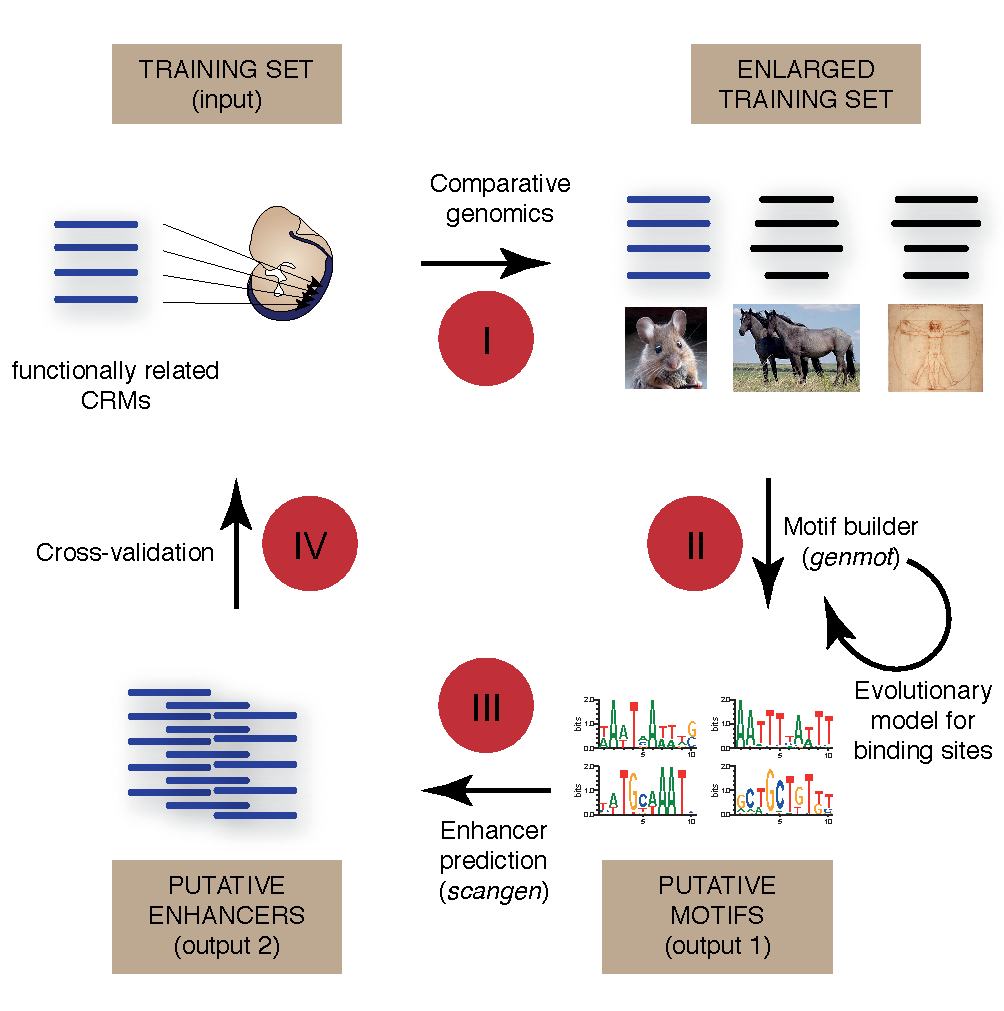
\includegraphics[width=15cm]{figuresnar-sub/fig1.pdf}
\end{center}
\caption{\normalsize
{\bf {\em Imogene} workflow.}
    The algorithm takes as input a list of functionally related CRMs.
    Homologous sequences from closely related species are automatically
    retrieved (I) and scanned in order to generate a list of putative
    transcription factor motifs (II).
    These motifs fuel the last step consisting in the inference of related
    novel CRMs (III).
    These predicted CRMs can finally be compared to a set of test CRMs to
    evaluate the predictability power  of the whole procedure (IV). 
    }
    \label{fig:workflow}
\end{figure}

\clearpage
\begin{figure}[!htbp]
\begin{center}
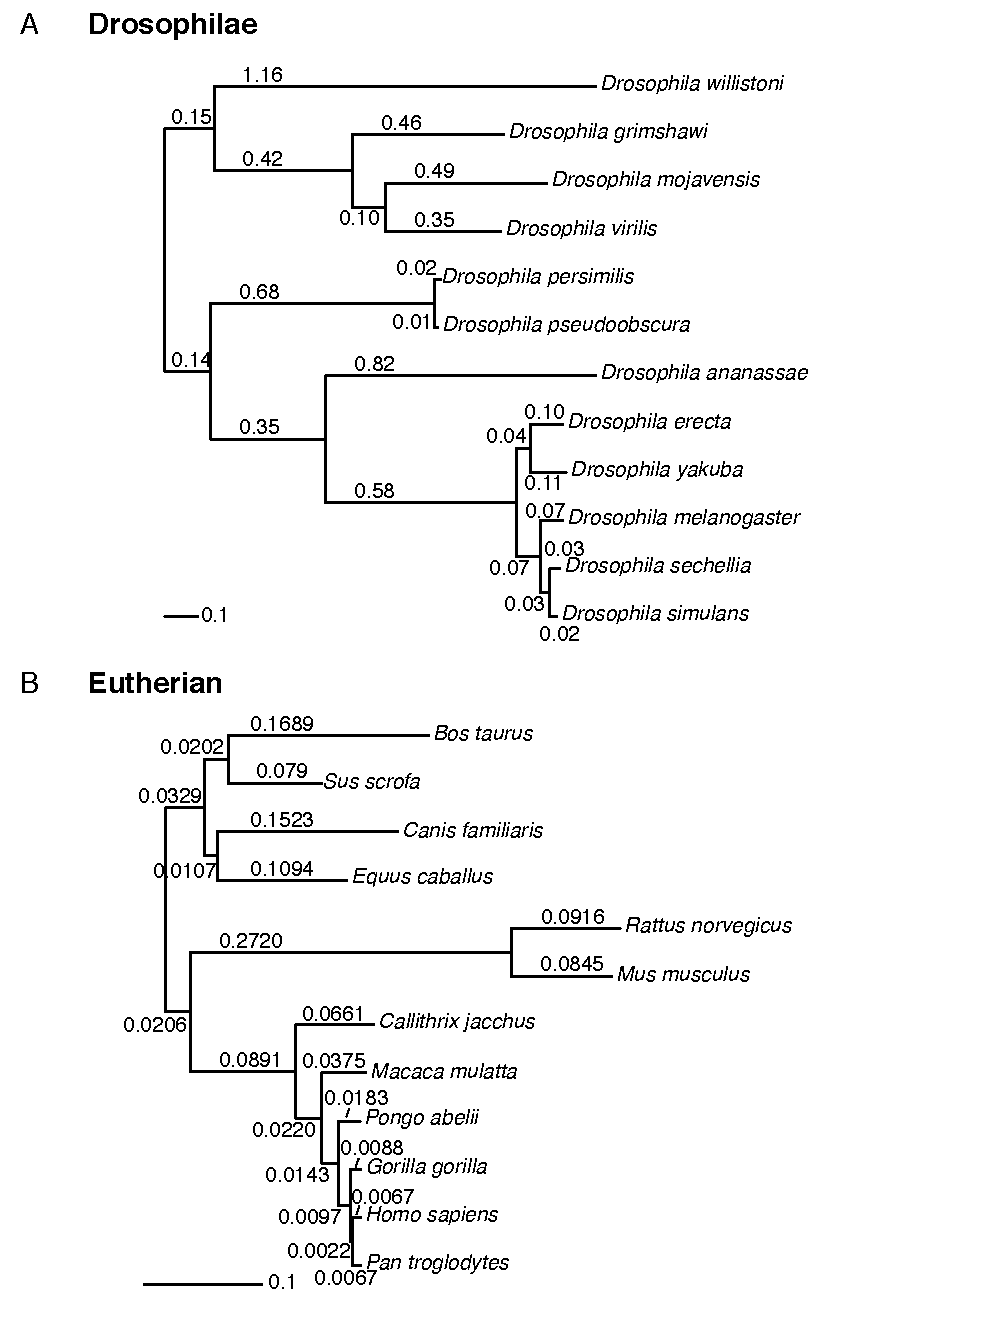
\includegraphics[width=15cm]{figuresnar-sub/fig2.pdf}
\end{center}
\caption{\normalsize
{\bf Phylogenetic trees and  phylogenetic distances used by {\em
    Imogene}}.
    The branch lengths represent the evolutionary distances $d$ used by the
evolutionary models at the motif construction stage.}
  \label{fig:tree}
\end{figure}

\clearpage
\begin{figure}[!htbp]
\begin{center}
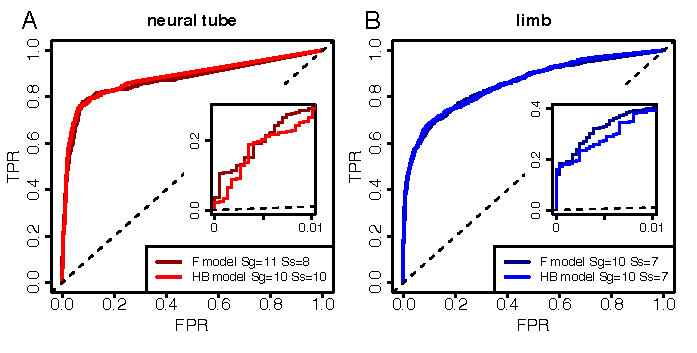
\includegraphics[width=15cm]{figuresnar-sub/fig3.pdf}
\end{center}
\caption{ \normalsize
    {\bf Analysis of well characterized developmental processes.}   	
    We tested the algorithm on mammal CRMs driving expression at E11.5 in
    neural tube (A) and limb (B). 
    For each class, CRMs were divided into a training set and a test set. 
    Motifs were learned on the training set and used to
    score CRMs from the test set along with background regions 
    consisting of the CRMs $1$kb flanking sequences (see { \em Methods}). 
    The displayed ROC curves show the proportion of test set CRMs recovered
    above a given score (True Positive Rate denoted by TPR) {\em vs.}
    the proportion of  recovered background sequence at the same score for the
    Felsenstein (F) and Halpern-Bruno (HB) models.
    The shown ROC plots are the results of 40 trials.
    The FPR $\leq1\%$ region of each curve is replotted in the insets for
    better visibility.
    For each test set and each evolutionary model, the thresholds $S_g$ and
    $S_s$ used for motifs generation and sequences scanning are given in the
    figures.
    Black dashed lines show random discrimination.  }
    \label{fig:mamtrain}
\end{figure}

\clearpage
    \begin{figure}[!htbp]
\begin{center}    
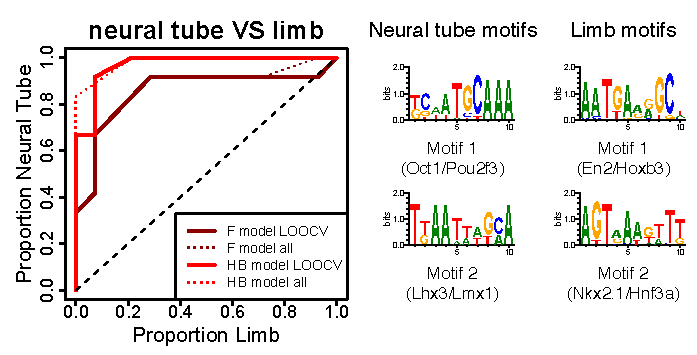
\includegraphics[width=15cm]{figuresnar-sub/fig4.pdf}
\end{center}
\caption{\normalsize
    {\bf Pattern recognition (mammals).} 
     ROC plots showing the discrimination between limb and neural CRMs using
     a simple linear classifier.
     Neural and limb classes are compared to each other. 
     Thick lines correspond to a leave-one-out cross-validation (LOOCV) scheme
     with a score function based on the {\it de novo} generated motifs from
     {\em Imogene}. 
     The results obtained with the two evolutionary models are shown
     (Felsenstein model (F) solid dark red line, with threshold parameters
     $S_g=11$, $S_s=9$, and Halpern-Bruno (HB) model, solid light red line,
     with threshold parameters $S_g=11$, $S_s=8$).
     The analogous discrimination curves based on learning motifs on  the whole
     training set (with the same threshold parameters) are shown for comparison
     (colored dashed lines). With this latter procedure, the discrimination is
     improved but still comparable to that computed by the LOOV, indicative of
     no strong overfitting of the training set. The corresponding
     discriminative motifs are shown for the whole training set learning with
     HB model (similar motifs are obtained with the F model).
     Black dashed line show random discrimination.  }   
    \label{fig:patternmam}
\end{figure}

\clearpage
    \begin{figure}[!htbp]
\begin{center}    
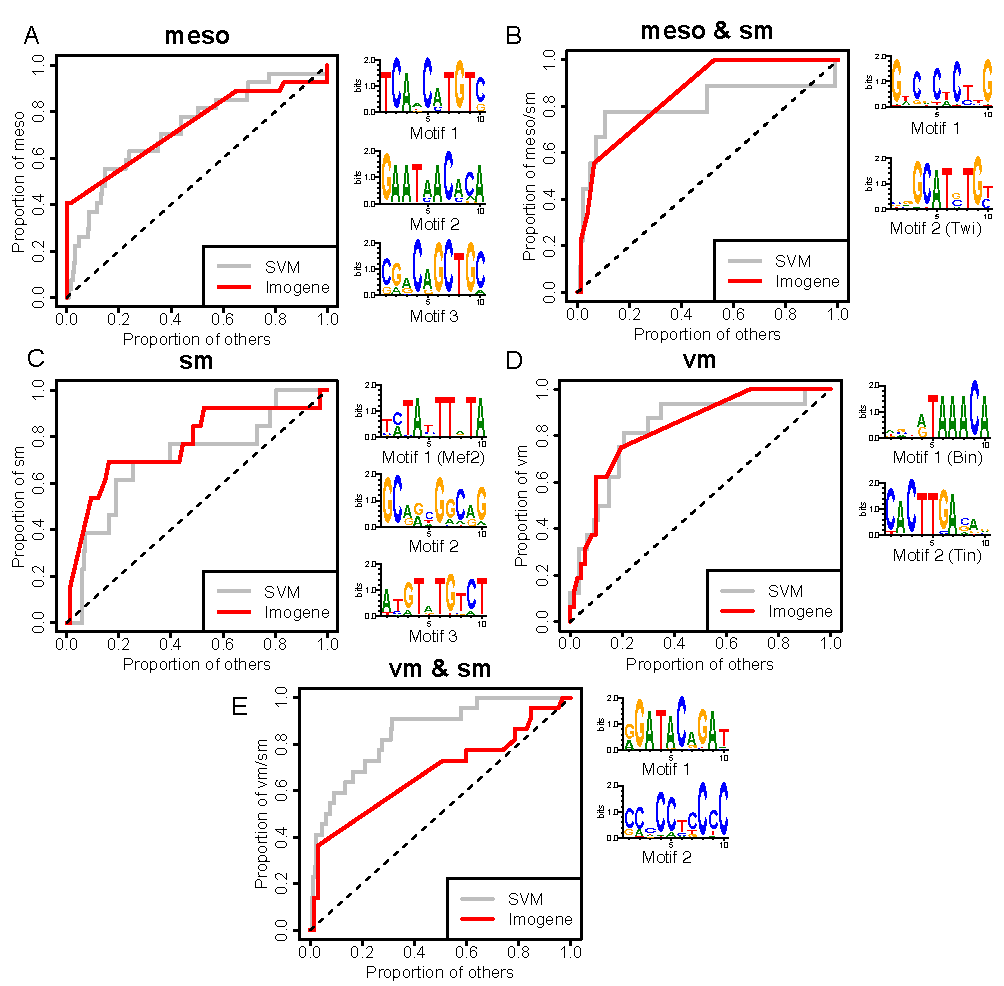
\includegraphics[width=15cm]{figuresnar-sub/fig5.pdf}
\end{center}
\caption{\normalsize
    {\bf Pattern recognition (Drosophilae).}     
    Recognition of classes of CRMs expressed in $5$ tissue types: mesoderm
    (meso), somatic muscle (sm), visceral muscle (vm) , mesoderm and somatic
    muscle (meso \& sm) and visceral and somatic muscle (vm \& sm).
    ROC plots are obtained using a leave-one-out cross-validation scheme.
    Two classifiers are compared: a Support Vector Machine using $15$ ChIPseq
    peak heights (grey, replotted using the data and the program provided in
    ref. \cite{pmid19890324}), and {\em Imogene} using the {\it de novo}
    generated motifs with Felsenstein evolutionary model (red) and a simple
    linear classifier (see {\em Methods}).
    The following thresholds were used: meso ($S_g=12$, $S_s=12$), meso \& sm
($S_g=10$, $S_s=10$), sm ($S_g=9$, $S_s=4$), vm ($S_g=10$, $S_s=10$), vm \& sm
($S_g=11$, $S_s=8$).  }
    \label{fig:patterndro}
\end{figure}

\clearpage
\begin{figure}[!htbp]
\begin{center} 
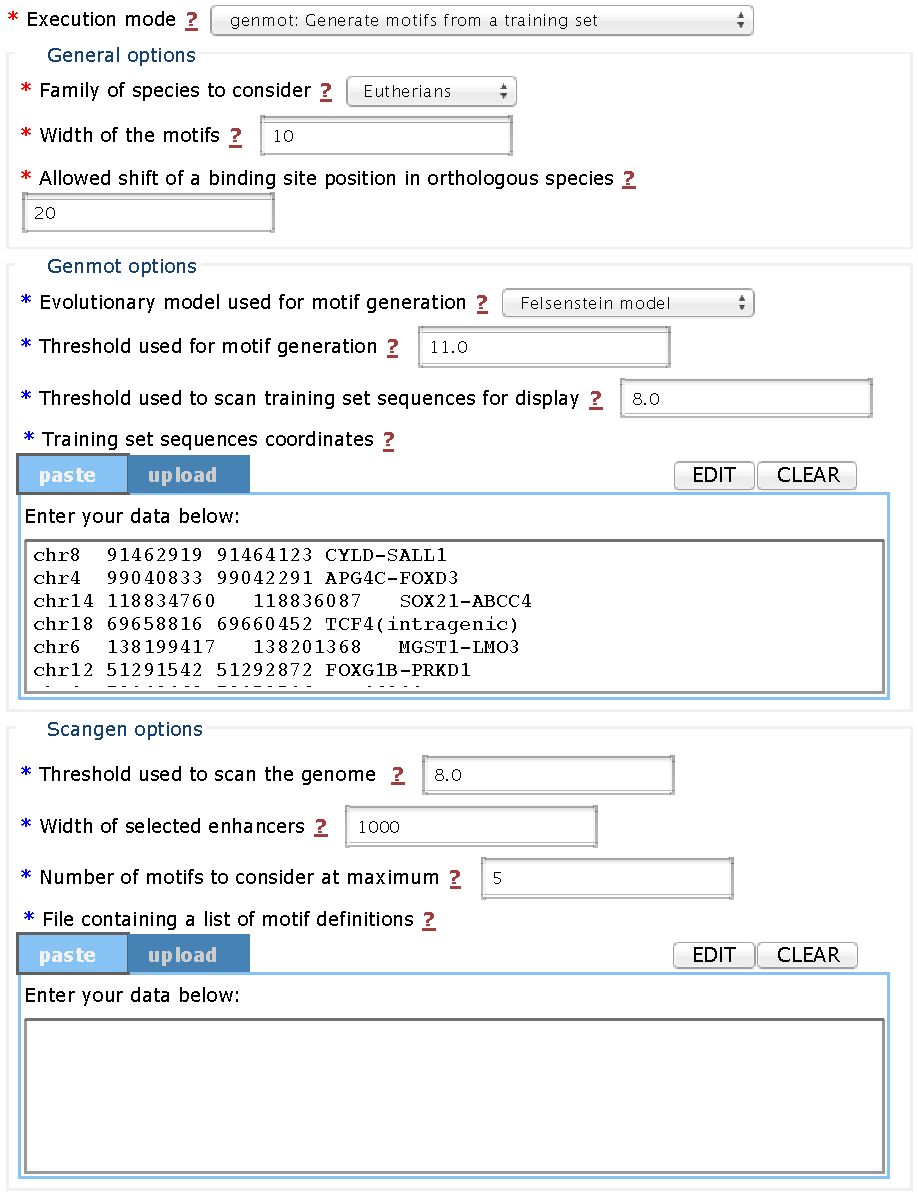
\includegraphics[width=15cm]{figuresnar-sub/fig6.pdf}
\end{center}
\caption{\normalsize
    {\bf Web based interface : input web page.} A copy 
    input web page for {\em Imogene} powered by the mobyle bioinformatics
    framework is shown. 
    }
    \label{fig:interfacein}
\end{figure}

\clearpage
        \begin{figure}[!htbp]
\begin{center} 
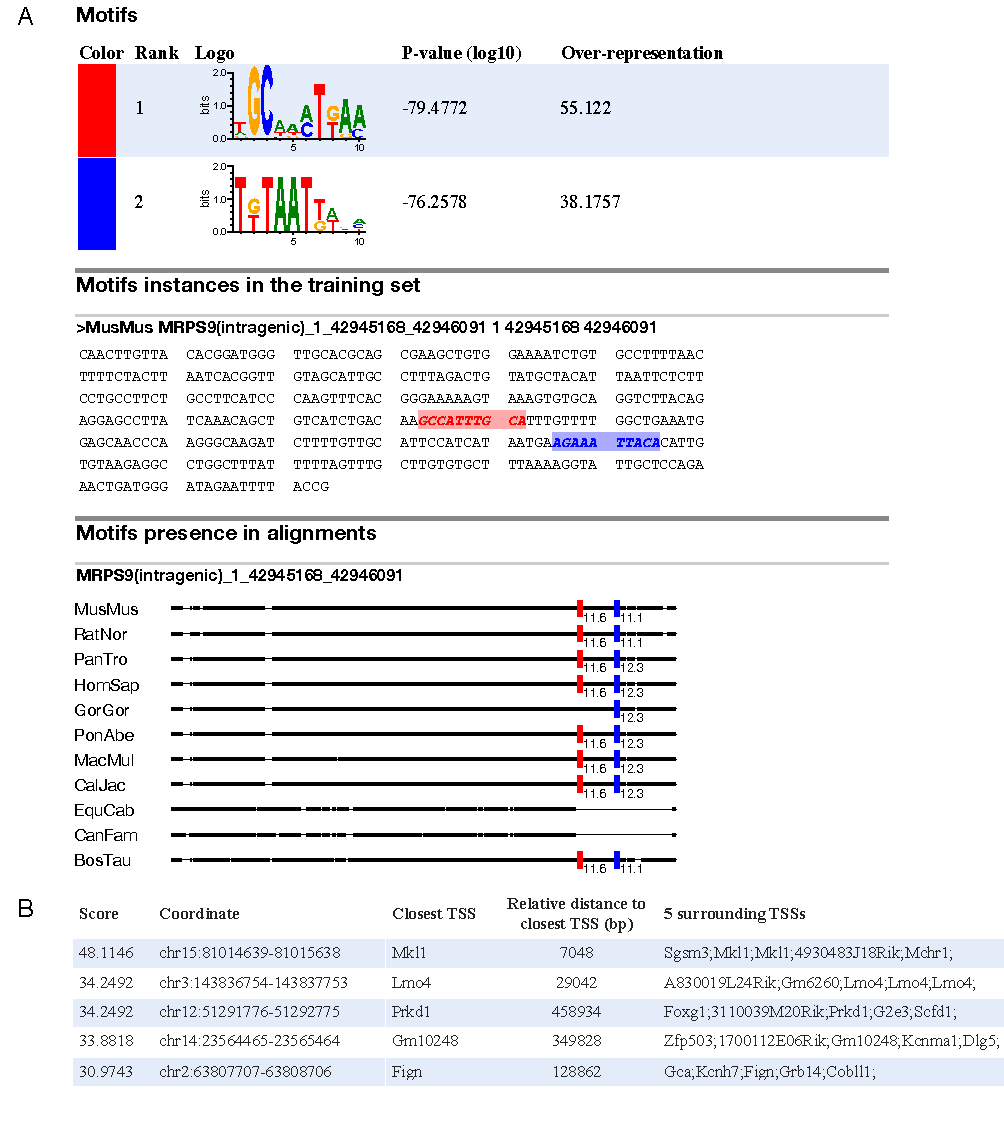
\includegraphics[width=15cm]{figuresnar-sub/fig7.pdf}
\end{center}
\caption{ \normalsize
{\bf Web based interface : output web page.}
    Example of an output web page for {\em Imogene} powered by the mobyle
    bioinformatics framework.
    A. Result page for the {\em Genmot} mode.
    Two motifs were generated from the neural tube full training set (default
    is $5$), using the same parameters as in Figure~\ref{fig:mamtrain}.
    Results are shown for the training set sequence MRPS9(intragenic). For
    display purposes, the beginning of the sequence, which contains no
    instances for the motifs, was cut in the middle panel. In the
    alignments, thick lines correspond to sequences and thin lines to gaps.
    B. Result page for the {\em Scangen} mode.
    The two generated motifs were used to score putative regulatory sequences
    of $1$kb in the mouse genome at optimal threshold $S_s=10$.
    The $5$ best ranking sequences are shown (default is $200$).}
    \label{fig:interfaceout}
\end{figure}


\clearpage  
  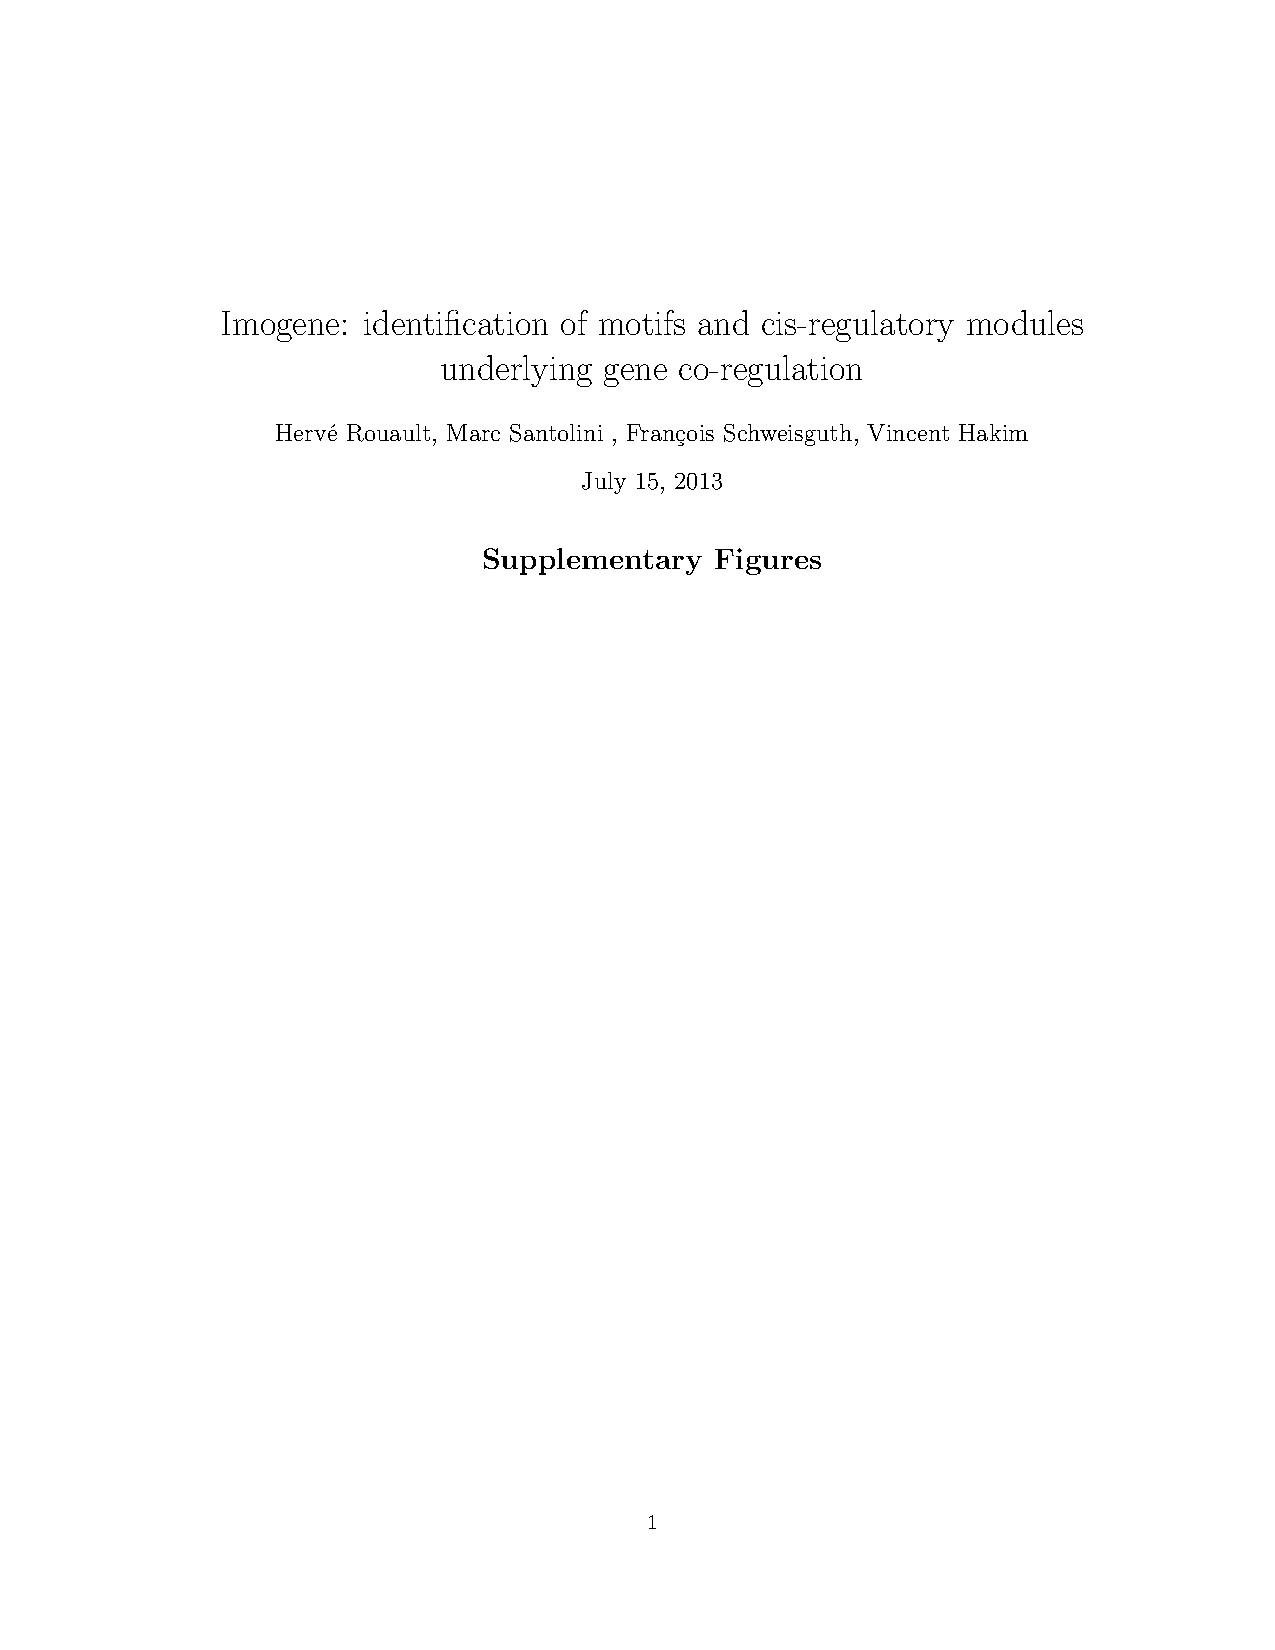
\includepdf[pages=-]{manuscriptSI.pdf}
  
\end{document}
